\section{ZLP subtraction and bandgap determination in WS$_2$}
\label{sec:results_sample}

Following the discussion of the vacuum results, we now move
to present the application of our fitting strategy to the parametrisation
of EEL spectra recorded on samples.
%
Specifically, we will analyse EELS measurements taken on the WS$_2$ nanostructures
presented in~\cite{SabryaWS2} and reviewed in Sect.~\ref{sec:tmd}.
%
These nanostructures exhibit a flower-like configuration where different layers
of material combine to form the petals and the stem of the flowers.
%
Their geometrical configuration is such that, depending on the specific region
of the nanostructure that one is imaging, the spectra will be sensitive
to different thicknesses and orientations of the material.

The parametrisation of these in-sample EEL spectra will then be used
to subtract the ZLP contribution and extract the bandgap energy $E_{\rm BG}$ from
the behaviour of $I_{\rm inel}(\Delta E)$ in the onset region.
%
The value of the bandgap  has been estimated in different ways
from subtracted EEL spectra, such as by means of the inflection point of the rising intensity or
a linear fit to the maximum positive slope~\cite{Schamm:2003}.
%
Here we will adopt the approach of~\cite{Rafferty:2000} whereby the behaviour
of $I_{\rm inel}(\Delta E)$ in the onset region is  modeled by
\begin{equation}
  \label{eq:I1}
    I_{\rm inel}(\Delta E) \simeq  A \lp \Delta E-E_{\rm BG} \rp^{b} \, , \quad \Delta E \ge E_{\rm BG} \, ,
\end{equation}
and vanishes for $E < E_{\rm BG}$, where $A$ and $b$ are constants extracted from the fit.
%
The power exponent $b$ is expected to be $b\simeq 1/2$ for a semiconductor material characterised
by a direct bandgap, and $b\simeq 3/2$ for the case instead of an indirect bandgap.

\subsection{Training dataset}
%
Fig.~\ref{fig:ws2positions} displays
low-magnification TEM images of two different regions of
the WS$_2$ nanoflowers, denoted as sample A and sample B in the following.
%
In each image we indicate the specific locations where
EEL spectra have been recorded, including in-vacuum measurements taken
for calibration purposes.
%
In the upper image, the differences in contrast are correlated to the material
thickness, with higher contrast corresponding to thinner regions.
%
Here the ZLP parametrisation strategy will be applied separately
to samples A and B, since in each case the EELS measurements have
been obtained with different electron microscopes and
operation settings, which thus as explained in Sect.~\ref{sec:eels}
must be analysed independently.

%%%%%%%%%%%%%%%%%%%%%%%%%%%%%%%%%%%%%%%%%%%%%%%%%%%%%%%%%%%%%%%%%%%%%%%
\begin{figure}[t]
\begin{centering}
  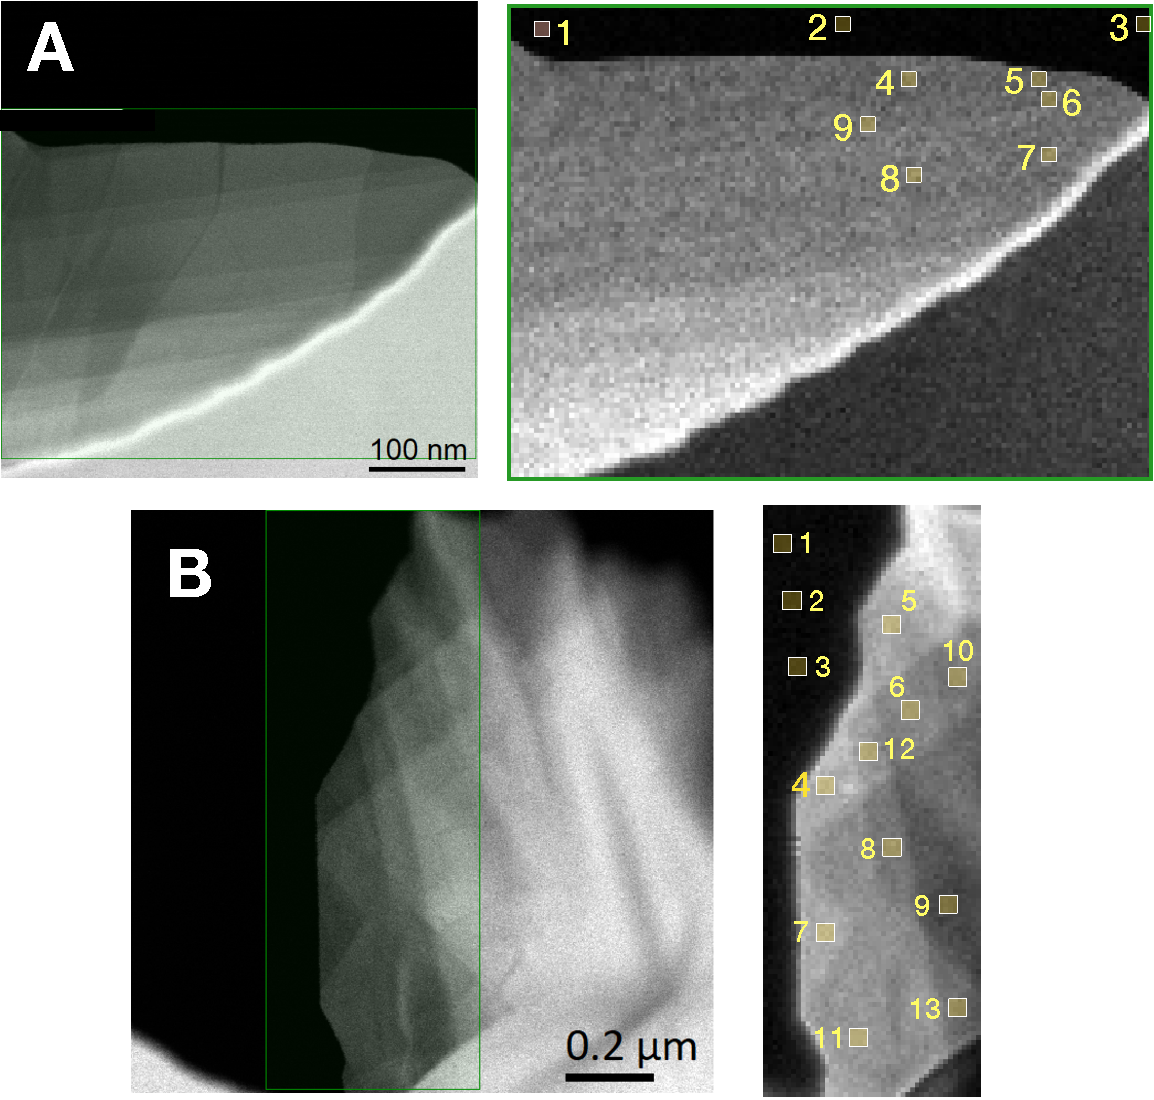
\includegraphics[width=0.87\linewidth]{plots/Spectra_location.pdf}
  \caption{Low-magnification TEM images of two different regions of
    the WS$_2$ nanoflowers, denoted as sample A and sample B respectively.
    %
    In each image we indicate the locations where
    EEL spectra have been recorded, including the in-vacuum measurements taken
    for calibration purposes.
    %
    In sample A the difference in contrast is correlated to the material
    thickness, with higher contrast corresponding to thinner regions of the nanostructure.
  }
\label{fig:ws2positions}
\end{centering}
\end{figure}
%%%%%%%%%%%%%%%%%%%%%%%%%%%%%%%%%%%%%%%%%%%%%%%%%%%%%%%%%%%%%%%%%%%%%%%%%%

In Table~\ref{table:sampledata} we collect the most relevant properties of the spectra collected
in the locations indicated in Fig.~\ref{fig:ws2positions} using the same convention as
in Table~\ref{table:sampledata}.
%
As mentioned, the sets of spectra from samples A and B
have been acquired with different microscopes and thus are
not directly comparable.
%
The full width at half maximum is averaged over all spectra of a given sample,
including those acquired on vacuum.
%
From this table one can observe that ....

%%%%%%%%%%%%%%%%%%%%%%%%%%%%%%%%%%%%%%%%%%%%%%%%%%%%%%%%%%%%%%%%%%%%%%%%%%%%%%%%%%%%%%%%%%%%%
%%%%%%%%%%%%%%%%%%%%%%%%%%%%%%%%%%%%%%%%%%%%%%%%%%%%%%%%%%%%%%%%%%%%%%%%%%%%%%%%%%%%%%%%%%%%%
\begin{table}[t]
  \begin{center}
            \renewcommand{\arraystretch}{1.50}
  \begin{tabular}{@{}ccccccccc}
\br
Set & $t_{\rm exp}$ {(}ms{)} & $E_{\rm b}$ {(}keV{)} & $N_{\rm sp}$ & $N_{\rm dat}$ & $\Delta E_{\rm min}$~(eV)  & $\Delta E_{\rm max}$~(eV)  & FWHM~(eV)  \\ 
\mr
A        &       ?       &    200 keV       &   11     &    2000    &     -0.93        & 9.07   & $\pm$         \\
B        &       ?       &        ?         &   6      &    1918    &     -4.054       & 45.471 & $ \pm$         \\
\br
  \end{tabular}
    \end{center}
  \caption{\small Same as Table~\ref{table:vacuumdata} now for the EEL spectra taken on WS$_2$ nanostructures.
  }
   \label{table:sampledata}
\end{table}
%%%%%%%%%%%%%%%%%%%%%%%%%%%%%%%%%%%%%%%%%%%%%%%%%%%%%%%%%%%%%%%%%%%%%%%%%%%%%%%%%%%%%%%%%%%%%%%%%5
%%%%%%%%%%%%%%%%%%%%%%%%%%%%%%%%%%%%%%%%%%%%%%%%%%%%%%%%%%%%%%%%%%%%%%%%%%%%%%%%%%%%%%%%%%%%%

In the following we will focus on representative spectra, specifically spectra \#4 and \#5 in sample
A and spectra \#14 and \#15 in sample B.
%
The full set of original spectra are made available together with the code used to
analyse them as described in this work, whose installation
and usage instructions are summarised in~\ref{sec:installation}.
%
By means of the {\tt Digital Micrograph} EELS software we can determine
the thickness of the material in each of the locations, and use it to
estimate the number of monolayers, taking into account that
one layer (S-W-S) of WS$_2$ has a thickness of around 0.9 nm.
%
For example, the thinner spectrum in sample A is \#5,
with a thickness of 2.1 nm corresponding to around 2 monolayers.

\subsection{ZLP subtraction}

In Table~\ref{table:sampledata_summary} we display
the mean value and uncertainty of the first local minima, $\Delta E|_{\rm min}$,
   averaged over the spectra corresponding to samples A and B from
    Fig.~\ref{fig:ws2positions},
as well as the corresponding values of the hyper-parameters
    $\Delta E_{\rm I}$ and $\Delta E_{\rm II}$ defined in Fig.~\ref{fig:EELS_toy}.
    %
Recall that as explained in Sect.~\ref{sec:methodology} only
the data with $\Delta E \le \Delta E_{\rm I}$ is used for the training
    of the neural network model.
    %
    For $\Delta E \ge \Delta E_{\rm II}$ instead, the training set includes only the pseudo-data
    that implements the $I_{\rm ZLP}(\Delta E)\to 0$ constraint.

%%%%%%%%%%%%%%%%%%%%%%%%%%%%%%%%%%%%%%%%%%%%%%%%%%%%%%%%%%%%%%%%%%%%%%%%%%%%%%%%%%%%%%%%%%%%%
%%%%%%%%%%%%%%%%%%%%%%%%%%%%%%%%%%%%%%%%%%%%%%%%%%%%%%%%%%%%%%%%%%%%%%%%%%%%%%%%%%%%%%%%%%%%%
\begin{table}[t]
  \begin{center}
            \renewcommand{\arraystretch}{1.50}
  \begin{tabular}{@{}ccccccccc}
\br
Set & $\Delta E|_{\rm min}$~(eV)  &  $\Delta E_{\rm I}$~(eV)  &  $\Delta E_{\rm II}$~(eV)   \\
\mr
A        &    $\pm$                &                   &              \\
B        &    $\pm$               &                     &               \\
\br
  \end{tabular}
    \end{center}
  \caption{\small The mean value and uncertainty of the first local minima, $\Delta E|_{\rm min}$,
    averaged over the spectra corresponding to samples A and B from
    Fig.~\ref{fig:ws2positions}.
    %
    We also indicate
     the corresponding values of the hyper-parameters
     $\Delta E_{\rm I}$ and $\Delta E_{\rm II}$ defined in Fig.~\ref{fig:EELS_toy} used for the training
     of the neural network model.
    %
  }
   \label{table:sampledata_summary}
\end{table}
%%%%%%%%%%%%%%%%%%%%%%%%%%%%%%%%%%%%%%%%%%%%%%%%%%%%%%%%%%%%%%%%%%%%%%%%%%%%%%%%%%%%%%%%%%%%%%%%%5
%%%%%%%%%%%%%%%%%%%%%%%%%%%%%%%%%%%%%%%%%%%%%%%%%%%%%%%%%%%%%%%%%%%%%%%%%%%%%%%%%%%%%%%%%%%%%

 We find that the location of the first minima is relatively stable
 among all the spectra belonging to given set.
 %
 The neural network training is performed for a wide range of $\Delta E_{\rm I}$ values
 subject to the condition that $\Delta E_{\rm I} \le \Delta E_{\rm min}$.
 %
 The optimal values listed  in Table~\ref{table:sampledata_summary} are selected
 by means of comparing the intensity derivatives in the sample with those
 of the vacuum combined with a stability analysis, as we discuss below.

 Upon completion of the neural network training, one ends up
 for each of the independent samples with
 a set $N_{\rm rep}=500$ replicas
 of the zero-loss peak parametrisation, $I_{\rm ZLP}^{({\rm mod})(k)}(\Delta E)$.
 %
 Assuming that we have $N_{\rm sp}$ spectra in each sample, then the zero-loss peak
 subtraction is performed individually
 for each Monte Carlo replica,
 \be
 \label{eq:subtractedModelPrediction}
 I_{\rm inel}^{({\rm mod})(j,k)}(\Delta E) \equiv I_{\rm EELS}^{(j)}(\Delta E) - I_{\rm ZLP}^{({\rm mod})(k)}(\Delta E)\, ,
 \quad \forall~N_{\rm rep} \, ,\quad j=1,\ldots,N_{\rm sp} \, ,
 \ee
 from which statistical estimators can be evaluated as usual.
 %
 For instance, the mean value for our model prediction for the $j$-th spectrum
 can be evaluated by averaging over the set of replicas,
 \be
 \la  I_{\rm inel}^{({\rm mod})(j)}\ra (\Delta E)
 = \frac{1}{N_{\rm rep}} \sum_{k=1}^{N_{\rm rep}}  I_{\rm inel}^{({\rm mod})(j,k)}(\Delta E) \, ,
 \quad j=1,\ldots,N_{\rm sp} \, ,
 \ee
 and likewise for the corresponding uncertainties.
%
 We note that for large values of $\Delta E$
 the model prediction reduces to the original spectra, since in that region
 the ZLP contribution vanishes by construction,
 \be
 I_{\rm inel}^{({\rm mod})(j,k)}(\Delta E \gg \Delta E_{\rm II}) \to  I_{\rm EELS}^{(j)}(\Delta E) \, ,\quad
 \forall~j,k \, .
 \ee
 
 For very small values of the energy loss $\Delta E$, the contribution to the total
 spectra from inelastic scatterings is negligible
 and thus the subtracted model prediction Eq.~(\ref{eq:subtractedModelPrediction}) should
 vanish.
 %
 However, this will not be the case in practice since the neural-net model is trained on
 the $N_{\rm sp}$ ensemble of spectra, rather that just on individual ones, and thus the expected
 $\Delta E \to 0$ behaviour will only be achieved within uncertainties rather than at the level of
 central values.
 %
 To achieve the desired $\Delta E \to 0$ limit, we apply a matching procedure
 as follows.
 %
 We introduce another hyper-parameter, $\Delta E_0 < \Delta E_1$, such that
 one has for the $k$-th ZLP replica associated to the $j$-th spectrum the following
 behaviour:
 \bea
 \nonumber
 I_{\rm ZLP}^{({\rm mod})(j,k)}(\Delta E) &=& I_{\rm EELS}^{(j)}(\Delta E) \, ,\quad \Delta E < \Delta E_0  \, ,\\
 I_{\rm ZLP}^{({\rm mod})(j,k)}(\Delta E) &=& I_{\rm EELS}^{(j)} + \lp \xi_1^{(n_l)(k)}(\Delta E) - I_{\rm EELS}^{(j)}(\Delta E)\rp  \times \mathcal{F} \, , \nonumber \quad 
 \Delta E_0 < \Delta E \le \Delta E_1 \, ,\\
 &&\mathcal{F} = \exp\lp -\frac{\lp \Delta E - \Delta E_1 \rp^2 }{\lp \Delta E_0 - \Delta E_1 \rp^2 \delta^2} \rp  \, , \label{eq:mathcing} \\
 I_{\rm ZLP}^{({\rm mod})(j,k)}(\Delta E) &=& \xi_1^{(n_l)(k)}(\Delta E) \, , \quad \Delta E > \Delta E_1 \nonumber \, ,
 \eea
 where $\xi_1^{(n_l)(k)}$ indicates the output of the $k$-th neural network that parametrises
 the ZLP and $\delta$ is a dimensionless tunable parameter.
 %
 In Eq.~(\ref{eq:mathcing}), $\mathcal{F}(\Delta E)$ represents a matching factor
 that ensures that the model prediction of the zero loss peak smoothly interpolates
 between $\Delta E=\Delta E_0$ (where $\mathcal{F}\ll 1$ and the original spectrum should
 be reproduced) and $\Delta E=\Delta E_1$
 (where $\mathcal{F}=1$ leaving the neural net output unmodified).
 %
 In  this work we choose $\Delta E_0 = \Delta E_1 -0.5\,{\rm eV}$, though we have verified
 that results are fairly independent of this choice.

 Taking into account the matching procedure, we can slightly modify Eq.~(\ref{eq:subtractedModelPrediction})
 to read
 \be
 \label{eq:subtractedModelPrediction2}
 I_{\rm inel}^{({\rm mod})(j,k)}(\Delta E) \equiv I_{\rm EELS}^{(j)}(\Delta E) - I_{\rm ZLP}^{({\rm mod})(j,k)}(\Delta E)\, ,
 \quad \forall~N_{\rm rep} \, ,\quad j=1,\ldots,N_{\rm sp} \, .
 \ee
 For each of the $N_{\rm sp}$ collected spectra and each of the $N_{\rm rep}$ replicas,
 we fit to Eq.~(\ref{eq:subtractedModelPrediction2}) the functional form Eq.~(\ref{eq:I1}).
 %
 The range in $\Delta E$ for these fits to the subtracted spectra is taken to be
 $\lc \Delta E_{\rm I} - 0.5~{\rm eV}, \Delta E_{\rm I} + 1.2~{\rm eV}\rc$.
 %
 This range has been chosen to maximise the amount of information in the onset region.
 %
 We end up, for each of the $N_{\rm sp}$ spectra, with $N_{\rm rep}$ values for
 the bandgap energy and fit exponent,
 \be
 \Big \{ E_{\rm BG}^{(j,k)}, b^{(j,k)} \Big\} \, , \quad k=1,\ldots,N_{\rm rep} \, ,
 \ee
 from which again one can evaluate statistical estimators such as medians, 68\% CL ranges,
 and correlations.

The left panel of Fig.~\ref{fig:sp4_subtracted_spectrum} displays
the original
and subtracted EEL spectrum corresponding to location \#4 in Fig.~\ref{fig:ws2positions},
together with the predictions of the ZLP model evaluated using
Eq.~(\ref{eq:mathcing}).
  %
Both for the ZLP model and for the subtracted spectrum we show both the central value
and the standard deviation of the predictions.
%
One can observe how uncertainties are negligible at low $\Delta E$
(due to the matching condition) and large $\Delta E$ (where the ZLP vanishes).
%
It is also possible to verify {\it a posteriori} that the choice of $\Delta E_I$
is sensible, by evaluating the following ratio
\be
\mathcal{R}_{\rm abs}\lp \Delta E_1\rp \equiv 
\la I_{\rm ZLP}^{({\rm mod})(j)}\ra /I_{\rm EELS}^{(j)} \Big|_{\Delta E = \Delta E1} \, .
\ee
One should verify that $\mathcal{R}_{\rm abs}\lp \Delta E_1\rp$ is not too far from unity,
indicating that the training dataset has not been contaminated by the inelastic contributions.
     

%%%%%%%%%%%%%%%%%%%%%%%%%%%%%%%%%%%%%%%%%%%%%%%%%%%%%%%%%%%%%%%%%%%%%%%
\begin{figure}[t]
\begin{centering}
  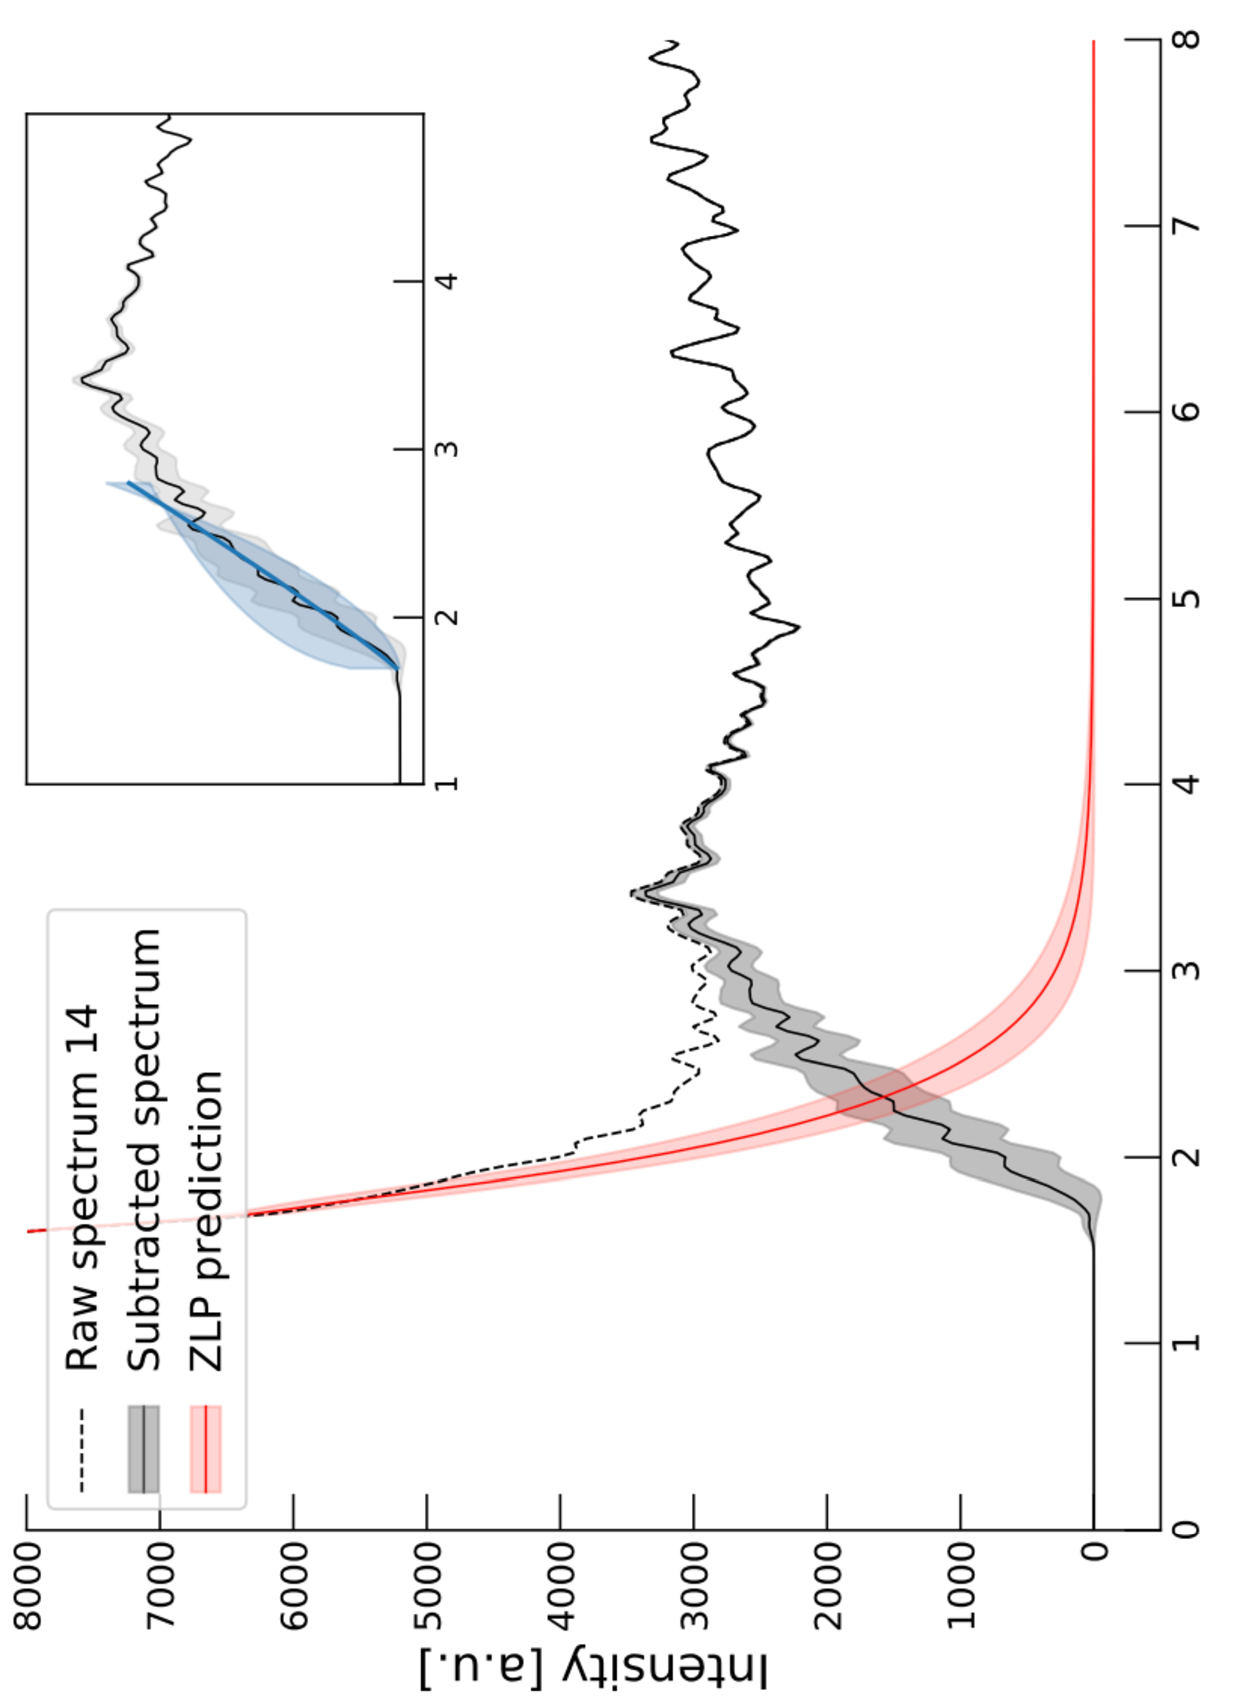
\includegraphics[width=0.36\linewidth,angle=-90]{plots/sp4_subtracted_spectrum.pdf}
   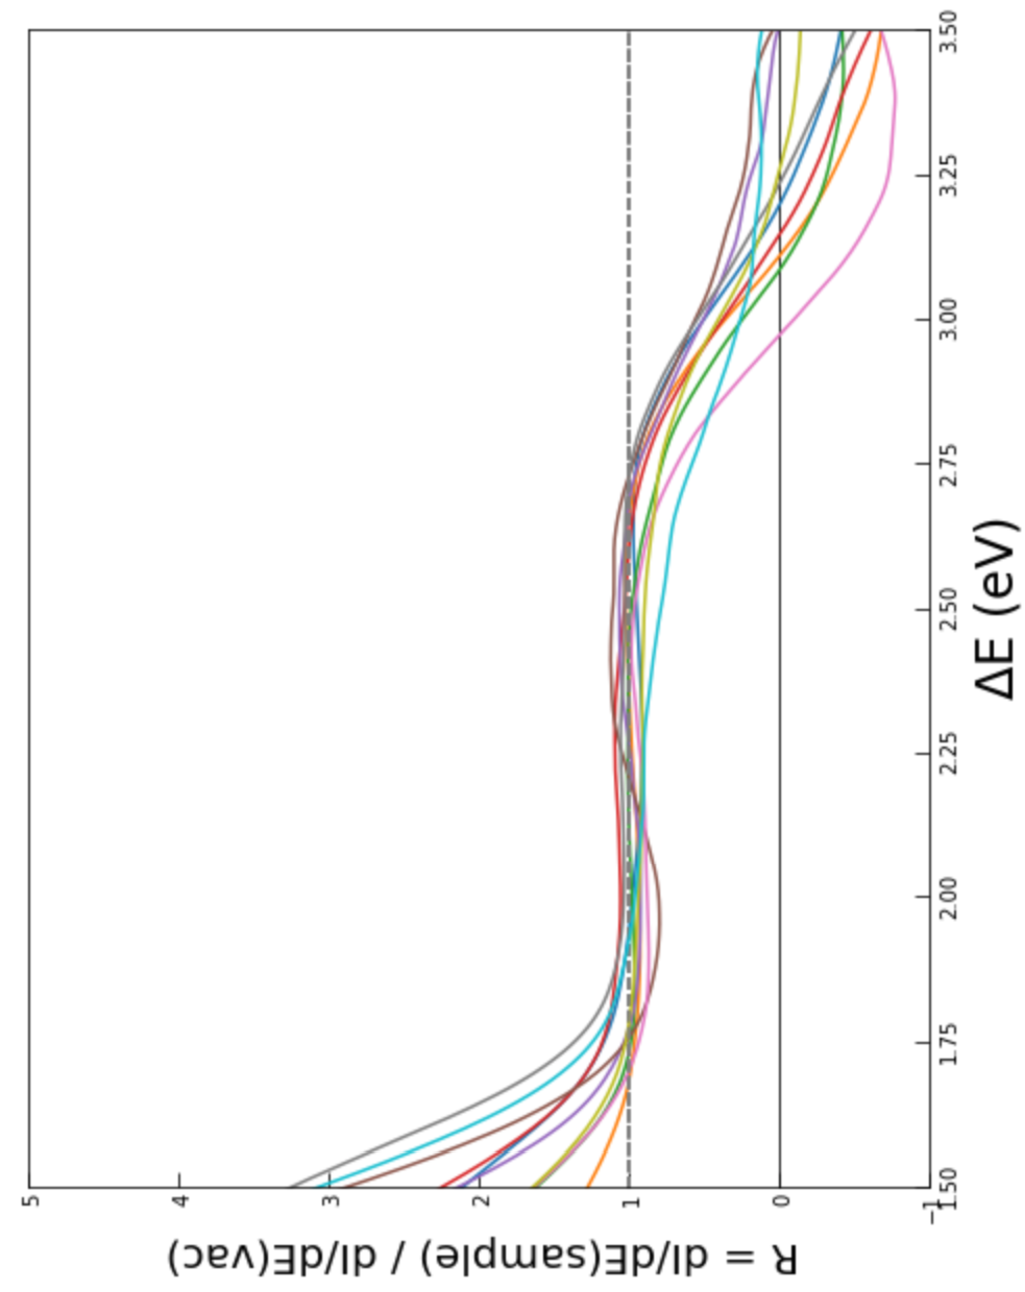
\includegraphics[width=0.36\linewidth,angle=-90]{plots/derivatives.pdf}
   \caption{Left: the original
     and subtracted EEL spectrum corresponding to location \#4 in Fig.~\ref{fig:ws2positions},
     together with the predictions of the ZLP models.
     %
     The inset displays the result of the fit using Eq.~(\ref{eq:I1}) to the onset
     region of the subtracted spectrum.
     %
     Right: The ratio of the derivative intensity of the original spectrum, $dI_{\rm EEL}/d\Delta E$,
     over that of the ZLP measurements taken on the vacuum $d I_{\rm ZLP}/d\Delta E$.
  }
\label{fig:sp4_subtracted_spectrum}
\end{centering}
\end{figure}
%%%%%%%%%%%%%%%%%%%%%%%%%%%%%%%%%%%%%%%%%%%%%%%%%%%%%%%%%%%%%%%%%%%%%%%%%%

The inset in the left panel of Fig.~\ref{fig:sp4_subtracted_spectrum}
shows the result of the  fits using Eq.~\ref{eq:I1} to the subtracted spectrum,
with the band indicating the 68\% CL uncertainties.
%
We discuss below the implication of this fit for the bandgap determination
in the WS$_2$ nanostructures.

In the right panel of  Fig.~\ref{fig:sp4_subtracted_spectrum} we display the ratio
between the derivative of the intensity profiles corresponding to the sample locations
with respect to a reference measurement taken on vacuum,
\be
\mathcal{R}_{\rm der}(\Delta E) \equiv 
\frac{
  dI_{\rm EELS}^{(j)}/ d\Delta E
}{
  dI_{\rm EELS}^{(j')} /d\Delta E
}\lp \Delta E\rp \, ,
\ee
where $j'$ labels one of the vacuum spectra.
%
This ratio allows to identify a suitable value of $\Delta E_{I}$ by determining
for which energy losses the derivatives of the sample spectra deviate significantly
from the vacuum ones.
%
Note that $\mathcal{R}_{\rm der}(\Delta E)=0$ indicates the position of the first
local minimum of the spectra.
%
From this comparison we can see that Fig.~\ref{fig:sp4_subtracted_spectrum} validates our choice of
$\Delta E_{\rm I}$.

\subsection{Bandgap determination}

We now move to discuss the results on the bandgap determination obtained
by fitting the functional form Eq.~(\ref{eq:I1}) to each of the subtracted
spectra defined by Eq.~(\ref{eq:subtractedModelPrediction2}).
%
Results will be presented as a function of the hyper-parameter $\Delta E_{\rm I}$
in order to gauge the stability of the results.
%
To begin with, in Fig.~\ref{fig:bvalues}
we display the values of the bandgap energy $E_{\rm BG}$ (top panels)
and of the exponent $b$ (bottom panels) as a function of $\Delta E_I$
for locations \#4 (left)
and \#5 (right panels) from Sample A indicated in Fig.~\ref{fig:ws2positions}.
%
The central value and the error band for each value of $\Delta E_I$ is evaluated
as the median and the 68\% CL interval over the $N_{\rm rep}=500$ Monte Carlo replicas.
%
The red marker indicates the position of the optimal value of
$\Delta E_{\rm I}$ determined as specified above.

%%%%%%%%%%%%%%%%%%%%%%%%%%%%%%%%%%%%%%%%%%%%%%%%%%%%%%%%%%
\begin{figure}[t]
\begin{centering}
  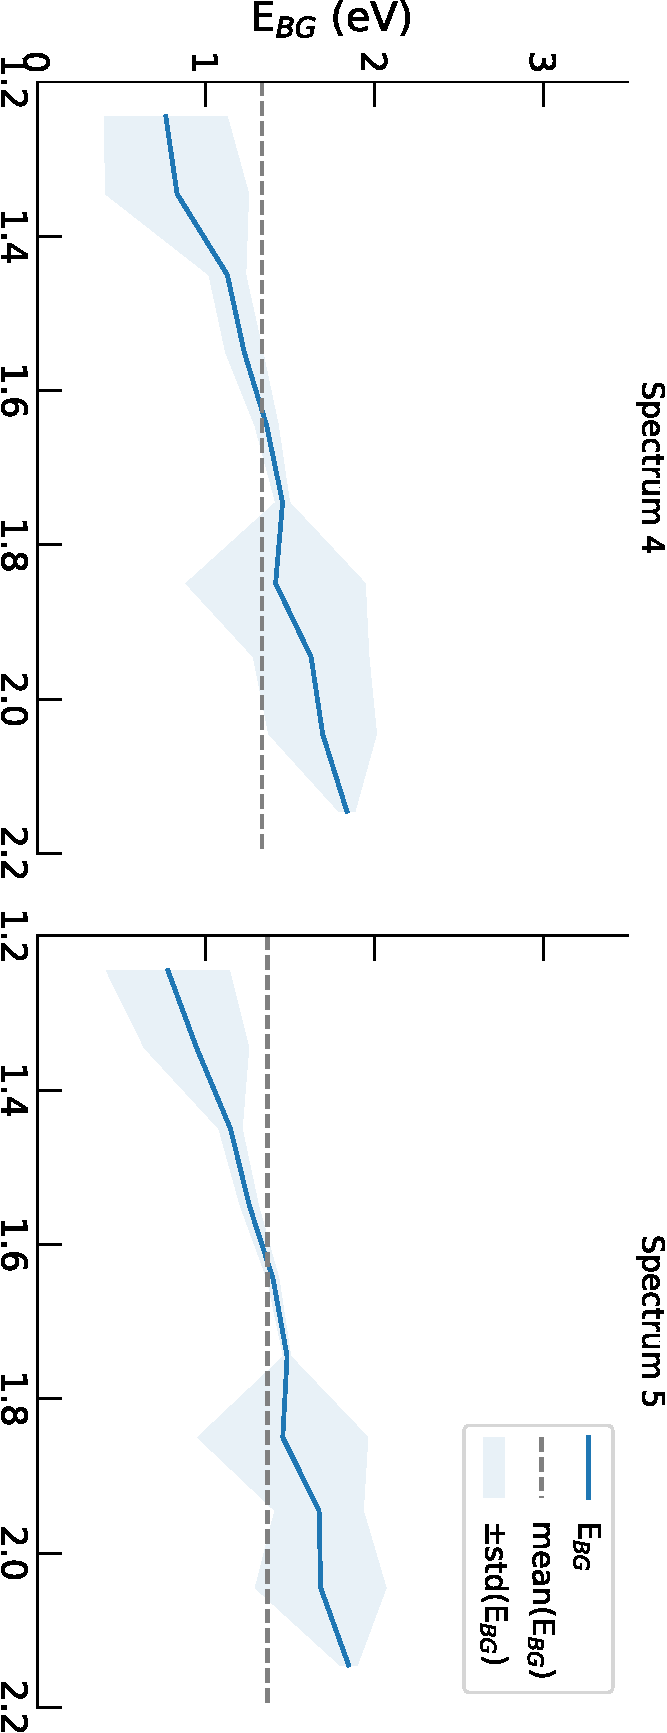
\includegraphics[width=0.38\linewidth,angle=90]{plots/bg_values_sampleA_sp4_sp5.pdf}
  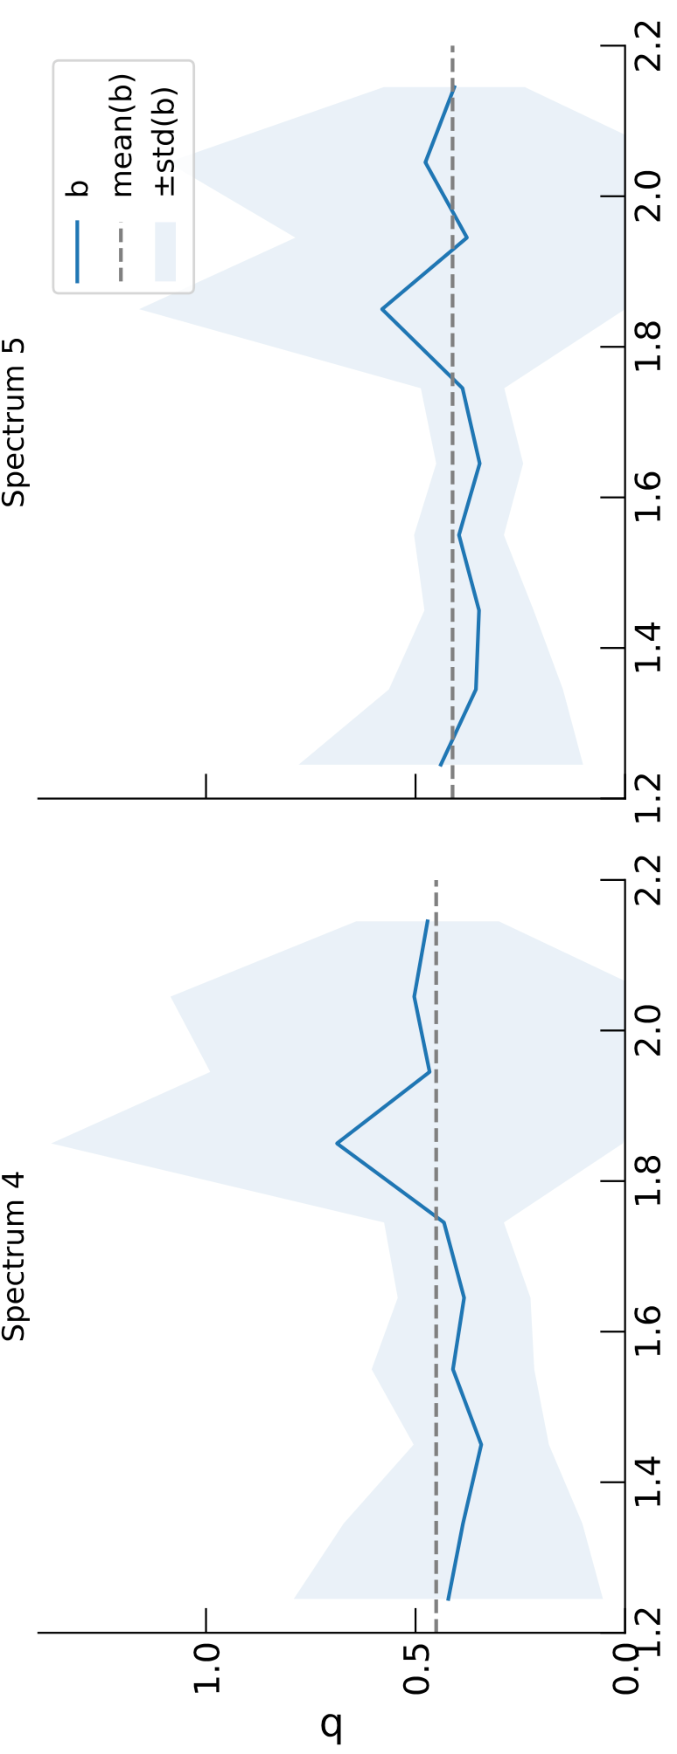
\includegraphics[width=0.38\linewidth,angle=-90]{plots/bvalues_sampleA_sp4_sp5.pdf} 
  \caption{Top: the values of the bandgap energy $E_{\rm BG}$ and of the exponent $b$
  obtained from fits to the onset
  region of subtracted spectra using Eq.~(\ref{eq:I1}) as a function
  of the hyper-parameter $\Delta E_{\rm I}$.
  %
  We show results for locations \#4 (left)
  and \#5 (right panels) from Sample A indicated in Fig.~\ref{fig:ws2positions}.
  %
  The central value and the error band for each value of $\Delta E_I$ is evaluated
  as the median and the 68\% CL interval over the $N_{\rm rep}=500$ Monte Carlo replicas.
  }
\label{fig:bvalues}
\end{centering}
\end{figure}
%%%%%%%%%%%%%%%%%%%%%%%%%%%%%%%%%%%%%%%%%%%%%%%%%%%%%%%%%%%%%

In Table~\ref{table:bandgap_fitting} we collect
 the median values and 68\% CL ranges for the bandgap energy $E_{\rm BG}$
 and the bandgap exponent $b$ determined from fitting Eq.~(\ref{eq:I1}) to each of the subtracted
 spectra defined by Eq.~(\ref{eq:subtractedModelPrediction2}).
 %
 We consider two representative spectra from sample A and two
 from sample B. 
 %
 The error is divided into the statistical and the systematic component, which are
 then added in quadrature to evaluate the total uncertainty in the fit results. 
 %
 From these results we see that the spectra in sample A are consistent with a direct bandgap,
 while those of sample B with an indirect bandgap.

%%%%%%%%%%%%%%%%%%%%%%%%%%%%%%%%%%%%%%%%%%%%%%%%%%%%%%%%%%%%%%%%%%%%%%%%%%%%%%%%%%%%%%%%%%%%%
%%%%%%%%%%%%%%%%%%%%%%%%%%%%%%%%%%%%%%%%%%%%%%%%%%%%%%%%%%%%%%%%%%%%%%%%%%%%%%%%%%%%%%%%%%%%%
\begin{table}[t]
  \begin{center}
    \footnotesize
            \renewcommand{\arraystretch}{1.50}
  \begin{tabular}{@{}c|c|c|c}
\br
Set & Spectrum   &$E_{\rm BG}$~(eV)  &  $b$  \\
\mr
\mr
A        &   sp\#4   &     $ 2.0 \pm 0.3^{\rm (stat)} \pm  0.2^{\rm (sys)}=  2.0 \pm 0.3^{\rm (tot)}   $                &       $ 0.5 \pm 0.3^{\rm (stat)} \pm  0.2^{\rm (sys)}=  0.5 \pm 0.3^{\rm (tot)}   $                       \\
\mr
A        &   sp\#5   &     $ 2.0 \pm 0.3^{\rm (stat)} \pm  0.2^{\rm (sys)}=  2.0 \pm 0.3^{\rm (tot)}   $                &       $ 0.5 \pm 0.3^{\rm (stat)} \pm  0.2^{\rm (sys)}=  0.5 \pm 0.3^{\rm (tot)}   $                       \\
\mr
\mr
B        &   sp\#14   &     $ 2.0 \pm 0.3^{\rm (stat)} \pm  0.2^{\rm (sys)}=  2.0 \pm 0.3^{\rm (tot)}   $                &       $ 0.5 \pm 0.3^{\rm (stat)} \pm  0.2^{\rm (sys)}=  0.5 \pm 0.3^{\rm (tot)}   $                       \\
\mr
B        &   sp\#15   &     $ 2.0 \pm 0.3^{\rm (stat)} \pm  0.2^{\rm (sys)}=  2.0 \pm 0.3^{\rm (tot)}   $                &       $ 0.5 \pm 0.3^{\rm (stat)} \pm  0.2^{\rm (sys)}=  0.5 \pm 0.3^{\rm (tot)}   $                       \\
\br
  \end{tabular}
    \end{center}
  \caption{\small The median values and 68\% CL ranges for the bandgap energy $E_{\rm BG}$
    and the bandgap exponent $b$ determined from fitting Eq.~(\ref{eq:I1}) to each of the subtracted
    spectra defined by Eq.~(\ref{eq:subtractedModelPrediction2}).
    %
    As justified in the text, we consider two representative spectra from sample A and two
    from sample B. 
    %
    The error is divided into the statistical and the systematic component, which are
    then added in quadrature to evaluate the total uncertainty in the fit results. {\rm ToDo}.
  }
   \label{table:bandgap_fitting}
\end{table}
%%%%%%%%%%%%%%%%%%%%%%%%%%%%%%%%%%%%%%%%%%%%%%%%%%%%%%%%%%%%%%%%%%%%%%%%%%%%%%%%%%%%%%%%%%%%%%%%%5
%%%%%%%%%%%%%%%%%%%%%%%%%%%%%%%%%%%%%%%%%%%%%%%%%%%%%%%%%%%%%%%%%%%%%%%%%%%%%%%%%%%%%%%%%%%%%
